<<<<<<< HEAD
\documentclass[11pt, a4paper]{article}
\usepackage[utf8x]{inputenc}
\usepackage[sort]{natbib}

\usepackage[spanish]{babel}
\usepackage{enumitem}
\usepackage{graphicx}
\usepackage{float}

\usepackage{etoolbox}

\usepackage{amsmath}
\usepackage{array}
\usepackage{gensymb}

\usepackage{fancyhdr}
\usepackage{multirow}
\usepackage{multicol}
\usepackage[table]{xcolor}
\usepackage{color}
\usepackage{colortbl}
\definecolor{lightgray}{gray}{0.9}
\setlength{\columnsep}{0.5cm}

\usepackage{tikz}
\usetikzlibrary{shapes.geometric, arrows}
\tikzstyle{problema} = [rectangle, rounded corners,  minimum width=3cm, minimum height=1cm,text centered, draw=black,fill={rgb:black,1;white,30}]
\tikzstyle{causa} = [rectangle, minimum width=3cm, minimum height=1cm, text centered, text width=4cm, draw=black, fill={rgb:black,0;white,10}]
\tikzstyle{nodo} = [diamond, minimum width=1cm, minimum height=1cm, text centered, draw=black, fill={rgb:black,0;white,10}]
\tikzstyle{arrow} = [thick,->,>=stealth]

\title{Titulo_TP_Elías,Hernando,Malerba,Miranda}

%------------------- Dimensiones -------------------
\usepackage{geometry}
\geometry{
	a4paper,				%tipo de papel
	textwidth = 160 mm,		%ancho del texto
	textheight = 237 mm,	%alto del texto
	inner = 30 mm,			%margen interno
	outer = 20 mm,			%margen externo
	voffset = 5 mm,			%separeción borde hoja - comienzo encabezado 
	headheight = 20 mm,		%alto del encabezado
	headsep = 5 mm,			%separación encabezado - texto
	footskip = 15 mm 		%separación textom - borde inf. pie de pág.
 }
%\usepackage{showframe} %muestra recuadro de los margenes definidos
%----------------------------------------------------

%------------------- Encabezado y Pie de pág -------------------
\fancyhead{}
\pagestyle{fancy}

\fancypagestyle{main}{%
	\fancyhf{}%
	\fancyhead[C]{	
		\begin{tabular}{cm{8cm} lm{4cm} cm{2cm}}
			\multirow{4}{2cm}{
\includegraphics[width=2cm]{Imagenes/UTN_logo}} &  & Elías, Tomás & 62510 \\
			& \centering Electrónica de Potencia & Hernando, Diego & 62509\\
			& \centering Trabajo Práctico N° 7: & Malerba, Iñaki & 63495 \\
			& \centering Control de velocidad para motor de CC & Miranda, Joaquín & 62513\\
		\end{tabular}
		}
%	\fancyhead[R]{Elías, Tomás 62510 \\ Hernando, Diego 62509\\ Malerba, Iñaki 63495 \\ Miranda, Joaquín 62513}
%	\fancyhead[C]{ Electrónica de Potencia \\ Trabajo Práctico N° 2 \\ Control del Ángulo de Disparo de un SCR }
%	\fancyhead[L]{
\includegraphics[width=1.8cm]{UTN_logo}}

	\fancyfoot{}
	\fancyfoot[R]{pág. \thepage}
	\fancyfoot[C]{Grupo: 2}
	\fancyfoot[L]{Curso: 5R1}
}

\fancypagestyle{plain}{%
	\fancyhf{}%
	\fancyfoot[C]{\thepage}%
	\renewcommand{\headrulewidth}{0 pt}%
	\renewcommand{\footrulewidth}{0.4pt}%
}
%----------------------------------------------------

\appto\frontmatter{\pagestyle{plain}}
\appto\mainmatter{\pagestyle{main}}

%----------------------------- Documento -----------------------------------------------
\begin{document}
	
	\begin{titlepage}
		% Capa
		\newcommand{\HRule}{\rule{\linewidth}{0.5mm}} % Defines a new command for the horizontal lines, change thickness here
		
		\center % Center everything on the page
		
		%----------------------------------------------------------------------------------------
		%	HEADING SECTIONS
		%----------------------------------------------------------------------------------------
		
		\textsc{\LARGE Universidad Tecnológica Nacional}\\[1cm] % Name of your university/college
		\textsc{\LARGE Facultad Regional Córdoba}\\[1cm] % Major heading such as course name
		\textsc{\Large Electrónica de Potencia}\\[2.5cm] % Minor heading such as course title
		
		%----------------------------------------------------------------------------------------
		%	TITLE SECTION
		%----------------------------------------------------------------------------------------
		
		\HRule \\[0.4cm]
		{\huge Trabajo Práctico N° 7 \\[0.5cm] \textbf{Control de Velocidad para motor de CC Lazo Abierto}}\\[0.4cm] % Title of your document
		\HRule \\[1.0cm]
		
		%----------------------------------------------------------------------------------------
		%	AUTHOR SECTION
		%----------------------------------------------------------------------------------------
		
		\vfill
		
		\begin{minipage}{0.805\textwidth}
			\begin{flushleft} \large
				\emph{Profesores:}\\
				Ing. \textsc {Oros}, Ramón\newline % Your name
				Ing. \textsc {Avramovich}, Javier\newline % Your name
			\end{flushleft}
		\end{minipage}\\[0.5cm]
			
		\begin{minipage}{0.4\textwidth}
			\begin{flushleft} \large
				\emph{Alumnos:}\\
				\textsc{Elías}, Tomás R. \newline % Your name
				\textsc{Hernando}, Diego J. \newline % Your name
				\textsc{Malerba}, Martin I.\newline % Your name
				\textsc{Miranda}, Joaquín M.\newline % Your name
			\end{flushleft}
		\end{minipage}
		~
		\begin{minipage}{0.4\textwidth}
			\begin{flushright} \large
				\emph{ } \\
				Leg 62510  \newline% Supervisor's Name
				Leg 62509  \newline% Supervisor's Name
				Leg 63495  \newline% Supervisor's Name
				Leg 62513  \newline% Supervisor's Name
			\end{flushright}
		\end{minipage}\\[1cm]
		
		{\large \today}\\ % Date, change the \today to a set date if you want to be precise
		% Fill the rest of the page with whitespace
		
	\end{titlepage}
	
	
	\frontmatter
	\newpage
	\tableofcontents
	\newpage
	
	\mainmatter

%----------------your title below -----------------------------

\section{Introducción}

Se denomina Puente H al circuito electrónico que permite a un motor de continua girar en ambos sentidos. Su nombre se debe a la disposición de los interruptores, que se observa en el esquema de la Figura \ref{fig:puenteH}

\begin{figure}[h]
	\centering
	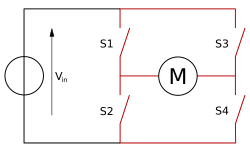
\includegraphics[width=6cm]{Imagenes/puenteH}
	\caption{Esquemático del Puente H.}
	\label{fig:puenteH}
\end{figure} 

El circuito funciona de la forma graficada en la Figura \ref{fig:puenteH_operacion}. Si consideramos el borne izquierdo del motor como el positivo, y el derecho como el negativo, cuando los interruptores S1 y S4 se cierran y S2 y S3 están abiertos, se aplica una tensión positiva en el motor, haciéndolo girar en un sentido. Invirtiendo esta configuración, es decir, abriendo los interruptores S1 y S4 y cerrando S2 y S3, el voltaje se invierte, logrando así que el motor gire en sentido inverso. 

Es importante remarcar que los interruptores de una misma rama no deben estar cerrados en un mismo instante de tiempo ya que ocasionarían un
corto circuito en la fuente de tensión. 

\begin{figure}[h]
	\centering
	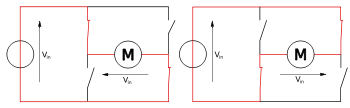
\includegraphics[width=13cm]{Imagenes/puenteH_operacion}
	\caption{Funcionamiento del Puente H.}
	\label{fig:puenteH_operacion}
\end{figure} 

Para lograr una modificación de la velocidad del motor -sin variar el par motriz- es necesario cambiar la tensión de alimentación del inducido sin modificar la corriente. Esto se logra con la modulación por ancho de pulso. 

La técnica de control mediante PWM se basa en la modificación del ciclo de trabajo de la señal que llega al controlador de los transistores que manejan la alimentación del motor, variando entre una conexión directa e inversa, donde la relación entre el ambos períodos determina el sentido y velocidad de giro del rotor.

Para lograr esto es necesario contar con 2 señales PWM complementarias que manejen una combinación de transistores cada una. En otras palabras, la suma de ambas señales debe significarle al motor un Dutty Cycle efectivo al motor lo mas cercano al 100\% posible, buscando así mantener el par motriz.


\section{Enunciado}
\begin{enumerate}
	\item Diseñar y construir un circuito que controle un motor de CC ( Ej. Mabuchi de 12V sin el regulador interno) en los cuatro cuadrantes con PWM y llave H con transistores MOSFET IRF830 con protección contra sobrecorrientes en el driver de compuerta, o en la llave H.
	
	El circuito será a lazo abierto. Tensión de referencia: +/- 5V (puede ser otro valor).
	
	Frecuencia de conmutación: 15khz, y contador de revoluciones con MOC70U1 (o equivalente)

	\item Efectuar las siguientes mediciones:
	\begin{enumerate}
		\item Graficar las RPM del motor en función de la tensión de referencia.
		\item Verificar funcionamiento del sist. de protección contra sobrecorrientes
	\end{enumerate}
\end{enumerate}

\section{Circuito}
\subsection{Actuador}


\begin{figure}[h]
	\centering
	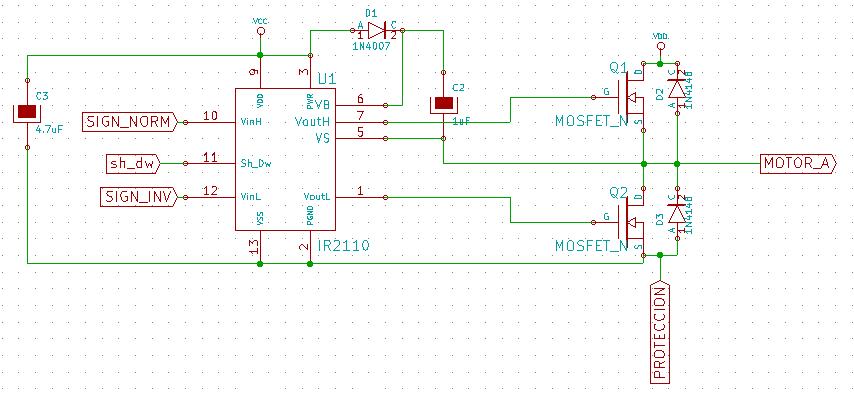
\includegraphics[width=13cm]{Imagenes/circ_driver.png}
	\caption{Medio puente H.}
	\label{fig:circ_driver}
\end{figure} 

El puente H está formado por 2 bloques simétricos, compuestos por dos transistores cada uno, controlados por un driver. Este circuito se puede observar en la Figura \ref{fig:circ_driver}.

\subsubsection{Transistores}

Para la realización del puente se utilizaron transistores MOSFET del tipo N modelo IRF830, como se solicita en la consigna. Estos transistores poseen un diodo conectado en paralelo que permiten a las corrientes circular en sentido inverso al previsto, situación que se da en la conmutación debido a las propiedades inductivas del bobinado del motor.

\subsubsection{Driver}
Para el control de los transistores se emplearon IR2110. Estos drivers poseen la particularidad de entregar dos salidas denominadas \textit{High Output} y \textit{Low Output}, de referencia independiente, lo que permite manejar ambos transistores de una rama con el mismo integrado.

Este bloque posee 3 entradas. Por un lado, las entradas \textit{SIGN\_NORM} y \textit{SIGN\_INV} serán las señales complementarias de PWM que exitarán al transistor superior e inferior respectivamente. Es necesario aclarar que en cada uno de los dos bloques \textit{"Puente H"} que componen el circuito, estas dos señales deben estar intercambiadas de posición para lograr el patrón de encendido y apagado de los transistores correctamente.

Adicionalmente a las dos señales de control, se encuentra la señal \textit{sh\_dw} -o Shutdown- que permite inhabilitar el driver. Esta señal la utilizaremos mas adelante en el bloque de protección (Sec. \ref{sec:proteccion}) para deshabilitar los motores ante una 
\textit{}


\subsection{Control}
\subsubsection{Generador de PWM}

Para este bloque utilizamos el integrado TL494. La principal característica de este integrado es la posibilidad de variar el ancho de pulso hasta un Dutty Cycle del 100\%. Para este caso, se calcularon los componentes para una frecuencia de trabajo de 15$kHz$ y luego se linealizó el potenciómetro $RV1$ mediante el cálculo de las resistencias $R1$ y $R2$, logrando una excursión completa.

Para la implementación utilizamos un preset para la regulación de la frecuencia, en la pata 6 del integrado, y un potenciómetro para la variación del ciclo de trabajo conectado al feedback.

La frecuencia de trabajo está dada por la constante de tiempo de los capacitores en las patas 5 y 6.

\begin{equation}
f_{osc} = \frac{1}{R * C} 
\end{equation}

Para la linealización medimos los valores de tensión de entrada \textit{FEEDBACK} del integrado que producían valores de dutty del 0\% y 100\%. En esta medición obtuvimos un dutty máximo con $3.5V$ y mínimo con $0.935V$, lo que nos permitió calcular que los valores de resistencia necesarios.

\begin{equation}
0.935V = \frac{5V}{1K\Omega + R_1 + R_2} * R_2
\end{equation}

\begin{equation}
3.5V  = \frac{5V}{1K\Omega + R_1 + R_2} * (1K\Omega + R_2)
\end{equation}

\begin{equation}
0.935 R_1 + (0.935 - 5) R_2 = -935
\end{equation}

\begin{equation}
3.5 R_1 + (3.5 - 5) R_2 = 1500
\end{equation}

\begin{equation}
R_1 = \frac{\Delta S_1}{\Delta p} = 584.8 \Omega
\end{equation}

\begin{equation}
R_2 = \frac{\Delta S_2}{\Delta p} = 364.52 \Omega
\end{equation}

Obtenidos estos valores, utilizamos $R_1$ = $560\Omega$ y $R_2$ = $363\Omega$ y obtuvimos un dutty entre 84\% y 12\%. Debido a esto, se modificaron ambos valores a $470\Omega$ y obtuvimos un dutty entre 97\% y 6\%.


\begin{figure}[h]
	\centering
	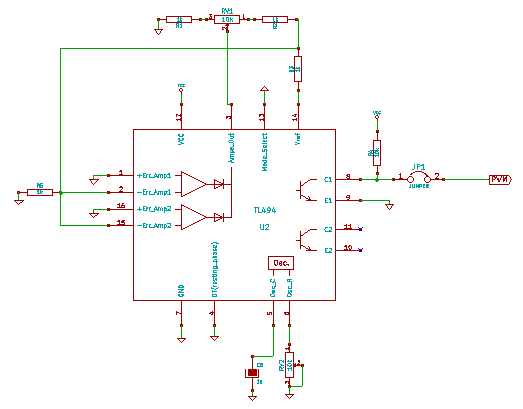
\includegraphics[width=13cm]{Imagenes/circ_pwm.png}
	\caption{Generador de PWM}
	\label{fig:circ_pwm}
\end{figure} 

\subsubsection{Generador de Tiempos Muertos}

El circuito generador de tiempos muertos ilustrado en la Figura \ref{fig:circ_retardo} es el encargado de generar un defasaje entre las señales de control, necesario para evitar que los dos transistores de la misma rama se exciten al mismo tiempo. 

Este tiempo muerto es necesario ya que los transistores poseen un tiempo entre el momento en el que la señal de control vuelve a 0 y el momento en el que se apagan. Este retardo se ilustra en la hoja de datos del transistor como \textit{Turn-Off Delay Time} $t_{off}$. Para garantizar una operación segura, exageramos este tiempo multiplicándolo por un factor de 10, debido a que las condiciones de funcionamiento no son iguales a las de utilizadas en las pruebas que realiza el fabricante, ni los transistores fabricados poseen exactas características entre si.

En el caso del IRF830, el $t_{off} = 42 ns$ por lo que utilizamos un tiempo muerto de aproximadamente $420ns$. 

\begin{equation}
\tau = R * C
\end{equation}

\begin{equation}
420 nS = R * 10 nF
\end{equation}

\begin{equation}
R = \frac{420 nS}{10 nF} = 42 \Omega
\end{equation}

En adición a la constante de tiempo utilizada para generar el retardo, es considerable el tiempo de propagación que posee la compuerta negadora, que en el caso del CD4049 es de $30nS$ c/u para $5V$.

El funcionamiento del circuito es el de un retardador con compuertas negadoras analizado en Técnicas Digitales I. Cuando en la entrada PWM hay un 0 lógico, a la salida de la primer compuerta obtenemos un 1 que cargará el capacitor rápidamente a través del diodo, lo que podrá un 1 en la entrada de la segunda compuerta y un 0 a la salida de la rama. Por otro lado, cuando a la entrada hay un 1, en la salida del primer inversor habrá un 0 que descargará el capacitor luego de un tiempo dado por el ajuste de la resistencia y el capacitor. Esto hará que la segunda compuerta demore en detectar el 0 retardando la aparición del 1 lógico a su salida.

La rama inferior incorpora una compuerta inversora extra, lo que invierte la señal produciendo la señal complementaria.



\begin{figure}[h]
	\centering
	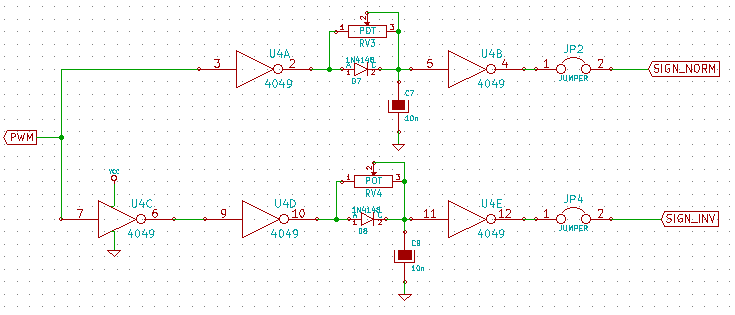
\includegraphics[width=13cm]{Imagenes/circ_retardo.png}
	\caption{Circuito de Retardo}
	\label{fig:circ_retardo}
\end{figure} 


\subsection{Protección}\label{sec:proteccion}

Para proteger el circuito de sobre corrientes, incluimos el bloque de protección detallado en la Figura \ref{fig:circ_protecc}.

A la salida del puente H, en serie con el motor, colocamos una resistencia sensora con el objetivo de medir la corriente que circula por el motor. Esta tensión medida, equivalente a la corriente, es comparada con una referencia fijada por un potenciómetro. A la salida del comparador, la señal resultante activa el pin de Shutdown \textit{sh\_dw} de los drivers.

Cuando la tensión en la resistencia sensora supera la tensión de referencia, la salida de comparador entrega una tensión equivalente a un 1 lógico que dispara el SCR poniendo en conducción el transistor BC558 que activa el pin de apagado de los IR2110, derivando en una inmediata interrupción de la alimentación de los motores. Gracias al circuito de enclavamiento generado por el SCR, es necesario interrumpir la excitación del transistor mediante el pulsador $SW1$ para que el SCR se apague y el motor vuelva a funcionar.

Para calibrar la protección se coloca el motor a girar a las revoluciones deseadas y se calibra para que, al aplicar fuerza extra sobre el eje, la protección se active. Esto garantiza un margen de corriente en el que el funcionamiento sea normal y que al aumentar la corriente, por un esfuerzo extra, la protección se active.


\begin{figure}[h]
	\centering
	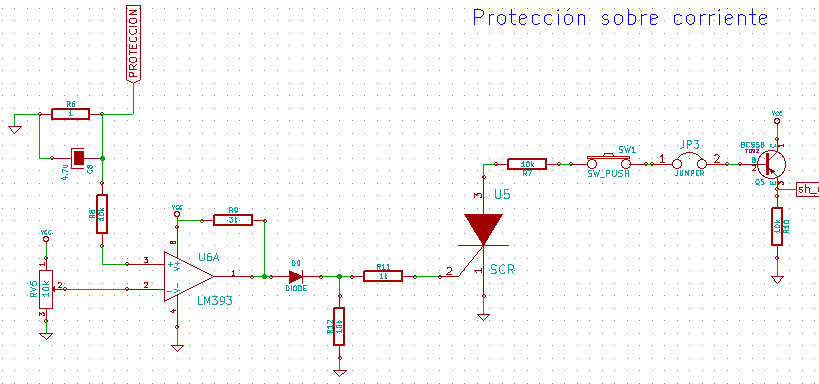
\includegraphics[width=13cm]{Imagenes/circ_prot.png}
	\caption{Circuito de Protección}
	\label{fig:circ_protecc}
\end{figure} 

\section{Mediciones}

En la Figura \ref{fig:osc_max} se observa el PWM obtenido para la condición de máxima velocidad del motor. En ella se puede apreciar los tiempos muertos entre ambas señales y el concepto del toque constante. 

Por otro lado, en la Figura \ref{fig:osc_min} ambas señales poseen un dutty cycle del 50\%, lo que provoca que el motor se detenga pero mantenga el torque.

\begin{figure}[h]
	\centering
	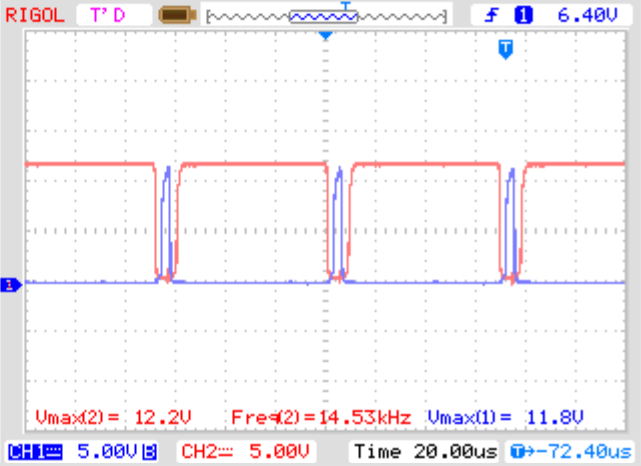
\includegraphics[width=9.5cm]{Imagenes/osc_max.png}
	\caption{PWM para motor a máxima velocidad}
	\label{fig:osc_max}
\end{figure} 



\begin{figure}[h]
	\centering
	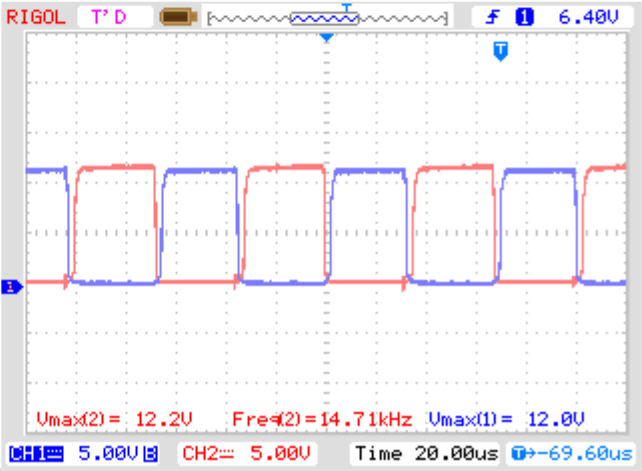
\includegraphics[width=9.5cm]{Imagenes/osc_min.png}
	\caption{PWM para detención del motor}
	\label{fig:osc_min}
\end{figure} 

\subsection{Volts vs RPM}
Mediante la utilización de un sensor infrarrojo y un marcador en el eje del motor procedimos a medir la relación entre la tensión de entrada al generador de PWM y las revoluciones por minuto obtenidas en el motor.

Para la relevación de las mediciones, barrimos manualmente el rango de funcionamiento de generador de señal y midiendo la frecuencia de los pulsos a la salida del sensor. Cada pulso negativo corresponde al momento en el que el sensor se veía obstruido por el marcador, por lo que la frecuencia en hertz obtenida es el equivalente a las RPS. Para obtener las RPM se multiplicó la medición por 60 segundos.

Los valores obtenidos fueron los siguientes:

%\begin{table}[]
%	\centering
%	\caption{Tensión vs RPM}
%	\label{my-label}
%	\begin{tabular}{l|l|l}
%
%
%Vref & Frec & RPM\\
%3,5	& 59,52	& 3571,2\\%
%3,4	& 53,19	& 3191,4\\
%3,3	& 48,1	& 2886\\
%3,2	& 42,37	& 2542,2\\
%3,1	& 37,8	& 2268\\
%3	& 31,65	& 1899\\
%2,9 & 25,51	& 1530,6\\
%2,8	& 19,69	& 1181,4\\
%2,7	& 14,53	& 871,8\\
%2,6	& 8,9	& 534\\
%2,5	& 2,8	& 168\\
%2,4	& 0	& 0\\
%1,9	& 0	& 0\\
%1,8	& 4,2	& 252\\
%1,7	& 6,3	& 378\\
%%1,6	& 11,63	& 697,8\\
%1,5	& 17,86	& 1071,6\\
%1,4	& 23,58	& 1414,8\\
%1,3	& 30,49	& 1829,4\\
%1,2	& 40,32	& 2419,2\\
%1,1	& 50	& 3000\\
%1	& 59,52	& 3571,2\\
%0,9	& 63,29	& 3797,4 \\
%	\end{tabular}
% \end{table}

\begin{figure}[h]
	\centering
	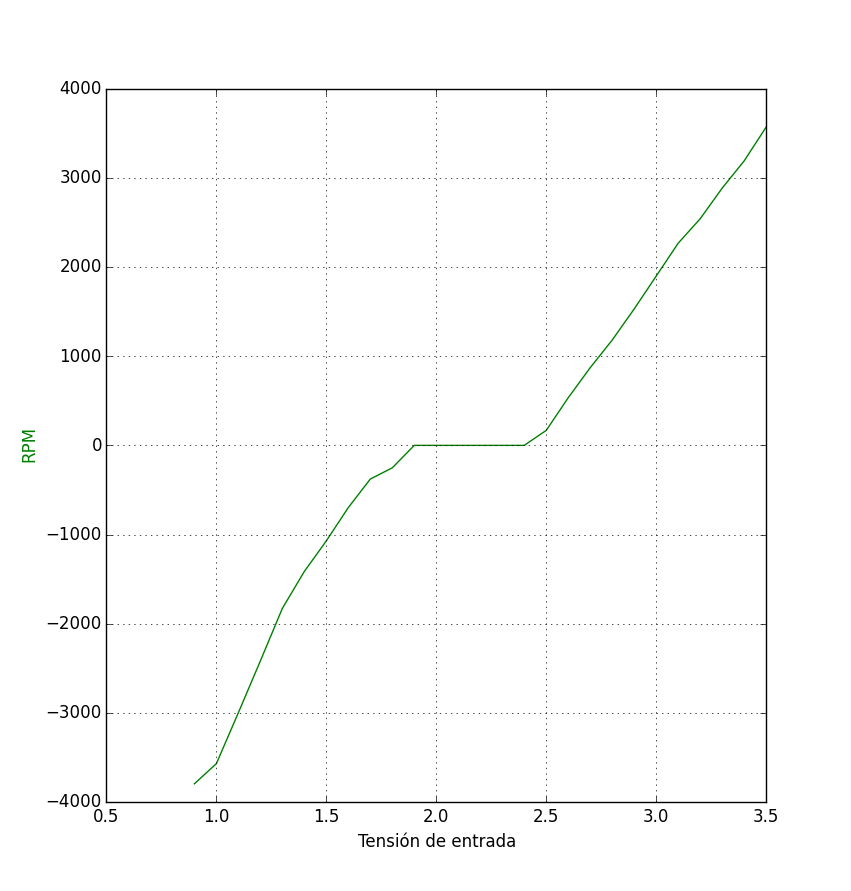
\includegraphics[width=15cm]{Imagenes/rpm.png}
	\caption{Curva de Tensión vs RPM}
	\label{fig:rpm}
\end{figure} 


\subsection{Protección}
Se ajustó la tensión de referencia en un valor tal que al forzar el motor, el circuito actuara y lo detuviera. La protección funcionó tal y como se esperaba, deteniendo la marcha hasta el momento en el que se presionó el pulsador de liberación.


\section{Conclusiones}
La implementación del circuito conllevó una dificultad mínima, logrando muy buenos resultados. El puente H resulta muy útil para controlar no solo la velocidad de giro, si no también el sentido de giro y lograr una frenada instantánea.

En este práctico, la señal de PWM la obtuvimos de un circuito integrado, controlando la velocidad mediante una señal de referencia, pero este circuito podría ser reemplazado por un microcontrolador y controlar la velocidad del motor digitalmente.

La separación del circuito en módulos permite la fabricación y prueba de los sub circuitos por separado. En nuestro caso utilizamos la protección por sobre corriente actuando sobre la pata de shutdown del driver, pero podríamos haber utilizado una implementación equivalente sobre la alimentación del circuito. Una variación al circuito de protección fue el agregado del SCR, que permite una mayor seguridad no volviendo a encender el motor hasta la intervención de un operario.

El potenciómetro nos permite ajustar el nivel de referencia para poder cambiar el nivel de protección, siendo capaces de ajustarlo al tipo de motor y a las necesidades de la aplicación

Al observar la curva de la relación Tensión - RPM, vemos un valle al cruzar por 0. Esto lo relacionamos al tamaño del motor, ya que un motor de tales dimensiones posee un umbral de tensión elevado para comenzar a moverse.


\end{document}
=======
\documentclass[11pt, a4paper]{article}
\usepackage[utf8x]{inputenc}
\usepackage[sort]{natbib}

\usepackage[spanish]{babel}
\usepackage{enumitem}
\usepackage{graphicx}
\usepackage{float}

\usepackage{etoolbox}

\usepackage{amsmath}
\usepackage{array}
\usepackage{gensymb}

\usepackage{fancyhdr}
\usepackage{multirow}
\usepackage{multicol}
\usepackage[table]{xcolor}
\usepackage{color}
\usepackage{colortbl}
\definecolor{lightgray}{gray}{0.9}
\setlength{\columnsep}{0.5cm}

\usepackage{tikz}
\usetikzlibrary{shapes.geometric, arrows}
\tikzstyle{problema} = [rectangle, rounded corners,  minimum width=3cm, minimum height=1cm,text centered, draw=black,fill={rgb:black,1;white,30}]
\tikzstyle{causa} = [rectangle, minimum width=3cm, minimum height=1cm, text centered, text width=4cm, draw=black, fill={rgb:black,0;white,10}]
\tikzstyle{nodo} = [diamond, minimum width=1cm, minimum height=1cm, text centered, draw=black, fill={rgb:black,0;white,10}]
\tikzstyle{arrow} = [thick,->,>=stealth]

\title{Titulo_TP_Elías,Hernando,Malerba,Miranda}

%------------------- Dimensiones -------------------
\usepackage{geometry}
\geometry{
	a4paper,				%tipo de papel
	textwidth = 160 mm,		%ancho del texto
	textheight = 237 mm,	%alto del texto
	inner = 30 mm,			%margen interno
	outer = 20 mm,			%margen externo
	voffset = 5 mm,			%separeción borde hoja - comienzo encabezado 
	headheight = 20 mm,		%alto del encabezado
	headsep = 5 mm,			%separación encabezado - texto
	footskip = 15 mm 		%separación textom - borde inf. pie de pág.
 }
%\usepackage{showframe} %muestra recuadro de los margenes definidos
%----------------------------------------------------

%------------------- Encabezado y Pie de pág -------------------
\fancyhead{}
\pagestyle{fancy}

\fancypagestyle{main}{%
	\fancyhf{}%
	\fancyhead[C]{	
		\begin{tabular}{cm{8cm} lm{4cm} cm{2cm}}
			\multirow{4}{2cm}{
\includegraphics[width=2cm]{Imagenes/UTN_logo}} &  & Elías, Tomás & 62510 \\
			& \centering Electrónica de Potencia & Hernando, Diego & 62509\\
			& \centering Trabajo Práctico N° 7: & Malerba, Iñaki & 63495 \\
			& \centering Control de velocidad para motor de CC & Miranda, Joaquín & 62513\\
		\end{tabular}
		}
%	\fancyhead[R]{Elías, Tomás 62510 \\ Hernando, Diego 62509\\ Malerba, Iñaki 63495 \\ Miranda, Joaquín 62513}
%	\fancyhead[C]{ Electrónica de Potencia \\ Trabajo Práctico N° 2 \\ Control del Ángulo de Disparo de un SCR }
%	\fancyhead[L]{
\includegraphics[width=1.8cm]{UTN_logo}}

	\fancyfoot{}
	\fancyfoot[R]{pág. \thepage}
	\fancyfoot[C]{Grupo: 2}
	\fancyfoot[L]{Curso: 5R1}
}

\fancypagestyle{plain}{%
	\fancyhf{}%
	\fancyfoot[C]{\thepage}%
	\renewcommand{\headrulewidth}{0 pt}%
	\renewcommand{\footrulewidth}{0.4pt}%
}
%----------------------------------------------------

\appto\frontmatter{\pagestyle{plain}}
\appto\mainmatter{\pagestyle{main}}

%----------------------------- Documento -----------------------------------------------
\begin{document}
	
	\begin{titlepage}
		% Capa
		\newcommand{\HRule}{\rule{\linewidth}{0.5mm}} % Defines a new command for the horizontal lines, change thickness here
		
		\center % Center everything on the page
		
		%----------------------------------------------------------------------------------------
		%	HEADING SECTIONS
		%----------------------------------------------------------------------------------------
		
		\textsc{\LARGE Universidad Tecnológica Nacional}\\[1cm] % Name of your university/college
		\textsc{\LARGE Facultad Regional Córdoba}\\[1cm] % Major heading such as course name
		\textsc{\Large Electrónica de Potencia}\\[2.5cm] % Minor heading such as course title
		
		%----------------------------------------------------------------------------------------
		%	TITLE SECTION
		%----------------------------------------------------------------------------------------
		
		\HRule \\[0.4cm]
		{\huge Trabajo Práctico N° 7 \\[0.5cm] \textbf{Control de Velocidad para motor de CC Lazo Abierto}}\\[0.4cm] % Title of your document
		\HRule \\[1.0cm]
		
		%----------------------------------------------------------------------------------------
		%	AUTHOR SECTION
		%----------------------------------------------------------------------------------------
		
		\vfill
		
		\begin{minipage}{0.805\textwidth}
			\begin{flushleft} \large
				\emph{Profesores:}\\
				Ing. \textsc {Oros}, Ramón\newline % Your name
				Ing. \textsc {Avramovich}, Javier\newline % Your name
			\end{flushleft}
		\end{minipage}\\[0.5cm]
			
		\begin{minipage}{0.4\textwidth}
			\begin{flushleft} \large
				\emph{Alumnos:}\\
				\textsc{Elías}, Tomás R. \newline % Your name
				\textsc{Hernando}, Diego J. \newline % Your name
				\textsc{Malerba}, Martin I.\newline % Your name
				\textsc{Miranda}, Joaquín M.\newline % Your name
			\end{flushleft}
		\end{minipage}
		~
		\begin{minipage}{0.4\textwidth}
			\begin{flushright} \large
				\emph{ } \\
				Leg 62510  \newline% Supervisor's Name
				Leg 62509  \newline% Supervisor's Name
				Leg 63495  \newline% Supervisor's Name
				Leg 62513  \newline% Supervisor's Name
			\end{flushright}
		\end{minipage}\\[1cm]
		
		{\large \today}\\ % Date, change the \today to a set date if you want to be precise
		% Fill the rest of the page with whitespace
		
	\end{titlepage}
	
	
	\frontmatter
	\newpage
	\tableofcontents
	\newpage
	
	\mainmatter

%----------------your title below -----------------------------

\section{Introducción}

Se denomina Puente H al circuito electrónico que permite a un motor de continua girar en ambos sentidos. Su nombre se debe a la disposición de los interruptores, que se observa en el esquema de la Figura \ref{fig:puenteH}

\begin{figure}[h]
	\centering
	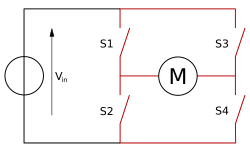
\includegraphics[width=6cm]{Imagenes/puenteH}
	\caption{Esquemático del Puente H.}
	\label{fig:puenteH}
\end{figure} 

El circuito funciona de la forma graficada en la Figura \ref{fig:puenteH_operacion}. Si consideramos el borne izquierdo del motor como el positivo, y el derecho como el negativo, cuando los interruptores S1 y S4 se cierran y S2 y S3 están abiertos, se aplica una tensión positiva en el motor, haciéndolo girar en un sentido. Invirtiendo esta configuración, es decir, abriendo los interruptores S1 y S4 y cerrando S2 y S3, el voltaje se invierte, logrando así que el motor gire en sentido inverso. 

Es importante remarcar que los interruptores de una misma rama no deben estar cerrados en un mismo instante de tiempo ya que ocasionarían un
corto circuito en la fuente de tensión. 

\begin{figure}[h]
	\centering
	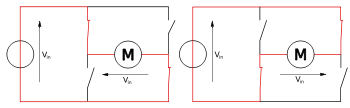
\includegraphics[width=13cm]{Imagenes/puenteH_operacion}
	\caption{Funcionamiento del Puente H.}
	\label{fig:puenteH_operacion}
\end{figure} 

Para lograr una modificación de la velocidad del motor -sin variar el par motriz- es necesario cambiar la tensión de alimentación del inducido sin modificar la corriente. Esto se logra con la modulación por ancho de pulso. 

La técnica de control mediante PWM se basa en la modificación del ciclo de trabajo de la señal que llega al controlador de los transistores que manejan la alimentación del motor, variando entre una conexión directa e inversa, donde la relación entre el ambos períodos determina el sentido y velocidad de giro del rotor.

Para lograr esto es necesario contar con 2 señales PWM complementarias que manejen una combinación de transistores cada una. En otras palabras, la suma de ambas señales debe significarle al motor un Dutty Cycle efectivo al motor lo mas cercano al 100\% posible, buscando así mantener el par motriz.


\section{Enunciado}
\begin{enumerate}
	\item Diseñar y construir un circuito que controle un motor de CC ( Ej. Mabuchi de 12V sin el regulador interno) en los cuatro cuadrantes con PWM y llave H con transistores MOSFET IRF830 con protección contra sobrecorrientes en el driver de compuerta, o en la llave H.
	
	El circuito será a lazo abierto. Tensión de referencia: +/- 5V (puede ser otro valor).
	
	Frecuencia de conmutación: 15khz, y contador de revoluciones con MOC70U1 (o equivalente)

	\item Efectuar las siguientes mediciones:
	\begin{enumerate}
		\item Graficar las RPM del motor en función de la tensión de referencia.
		\item Verificar funcionamiento del sist. de protección contra sobrecorrientes
	\end{enumerate}
\end{enumerate}

\section{Circuito}
\subsection{Actuador}


\begin{figure}[h]
	\centering
	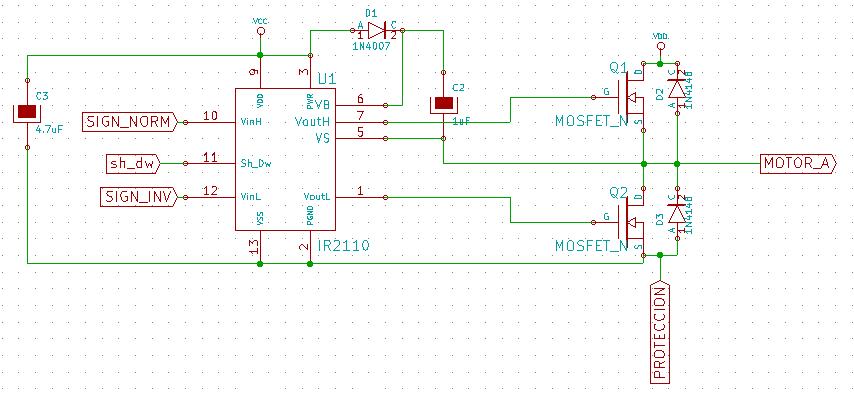
\includegraphics[width=13cm]{Imagenes/circ_driver.png}
	\caption{Medio puente H.}
	\label{fig:circ_driver}
\end{figure} 

El puente H está formado por 2 bloques simétricos, compuestos por dos transistores cada uno, controlados por un driver. Este circuito se puede observar en la Figura \ref{fig:circ_driver}.

\subsubsection{Transistores}

Para la realización del puente se utilizaron transistores MOSFET del tipo N modelo IRF830, como se solicita en la consigna. Estos transistores poseen un diodo conectado en paralelo que permiten a las corrientes circular en sentido inverso al previsto, situación que se da en la conmutación debido a las propiedades inductivas del bobinado del motor.

\subsubsection{Driver}
Para el control de los transistores se emplearon IR2110. Estos drivers poseen la particularidad de entregar dos salidas denominadas \textit{High Output} y \textit{Low Output}, de referencia independiente, lo que permite manejar ambos transistores de una rama con el mismo integrado.

Este bloque posee 3 entradas. Por un lado, las entradas \textit{SIGN\_NORM} y \textit{SIGN\_INV} serán las señales complementarias de PWM que exitarán al transistor superior e inferior respectivamente. Es necesario aclarar que en cada uno de los dos bloques \textit{"Puente H"} que componen el circuito, estas dos señales deben estar intercambiadas de posición para lograr el patrón de encendido y apagado de los transistores correctamente.

Adicionalmente a las dos señales de control, se encuentra la señal \textit{sh\_dw} -o Shutdown- que permite inhabilitar el driver. Esta señal la utilizaremos mas adelante en el bloque de protección (Sec. \ref{sec:proteccion}) para deshabilitar los motores ante una 
\textit{}


\subsection{Control}
\subsubsection{Generador de PWM}

Para este bloque utilizamos el integrado TL494. La principal característica de este integrado es la posibilidad de variar el ancho de pulso hasta un Dutty Cycle del 100\%. Para este caso, se calcularon los componentes para una frecuencia de trabajo de 15$kHz$ y luego se linealizó el potenciómetro $RV1$ mediante el cálculo de las resistencias $R1$ y $R2$, logrando una excursión completa.

Para la implementación utilizamos un preset para la regulación de la frecuencia, en la pata 6 del integrado, y un potenciómetro para la variación del ciclo de trabajo conectado al feedback.

La frecuencia de trabajo está dada por la constante de tiempo de los capacitores en las patas 5 y 6.

\begin{equation}
f_{osc} = \frac{1}{R * C} 
\end{equation}

Para la linealización medimos los valores de tensión de entrada \textit{FEEDBACK} del integrado que producían valores de dutty del 0\% y 100\%. En esta medición obtuvimos un dutty máximo con $3.5V$ y mínimo con $0.935V$, lo que nos permitió calcular que los valores de resistencia necesarios.

\begin{equation}
0.935V = \frac{5V}{1K\Omega + R_1 + R_2} * R_2
\end{equation}

\begin{equation}
3.5V  = \frac{5V}{1K\Omega + R_1 + R_2} * (1K\Omega + R_2)
\end{equation}

\begin{equation}
0.935 R_1 + (0.935 - 5) R_2 = -935
\end{equation}

\begin{equation}
3.5 R_1 + (3.5 - 5) R_2 = 1500
\end{equation}

\begin{equation}
R_1 = \frac{\Delta S_1}{\Delta p} = 584.8 \Omega
\end{equation}

\begin{equation}
R_2 = \frac{\Delta S_2}{\Delta p} = 364.52 \Omega
\end{equation}

Obtenidos estos valores, utilizamos $R_1$ = $560\Omega$ y $R_2$ = $363\Omega$ y obtuvimos un dutty entre 84\% y 12\%. Debido a esto, se modificaron ambos valores a $470\Omega$ y obtuvimos un dutty entre 97\% y 6\%.


\begin{figure}[h]
	\centering
	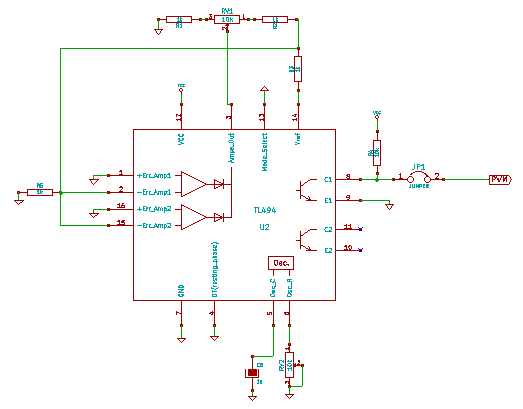
\includegraphics[width=13cm]{Imagenes/circ_pwm.png}
	\caption{Generador de PWM}
	\label{fig:circ_pwm}
\end{figure} 

\subsubsection{Generador de Tiempos Muertos}

El circuito generador de tiempos muertos ilustrado en la Figura \ref{fig:circ_retardo} es el encargado de generar un defasaje entre las señales de control, necesario para evitar que los dos transistores de la misma rama se exciten al mismo tiempo. 

Este tiempo muerto es necesario ya que los transistores poseen un tiempo entre el momento en el que la señal de control vuelve a 0 y el momento en el que se apagan. Este retardo se ilustra en la hoja de datos del transistor como \textit{Turn-Off Delay Time} $t_{off}$. Para garantizar una operación segura, exageramos este tiempo multiplicándolo por un factor de 10, debido a que las condiciones de funcionamiento no son iguales a las de utilizadas en las pruebas que realiza el fabricante, ni los transistores fabricados poseen exactas características entre si.

En el caso del IRF830, el $t_{off} = 42 ns$ por lo que utilizamos un tiempo muerto de aproximadamente $420ns$. 

\begin{equation}
\tau = R * C
\end{equation}

\begin{equation}
420 nS = R * 10 nF
\end{equation}

\begin{equation}
R = \frac{420 nS}{10 nF} = 42 \Omega
\end{equation}

En adición a la constante de tiempo utilizada para generar el retardo, es considerable el tiempo de propagación que posee la compuerta negadora, que en el caso del CD4049 es de $30nS$ c/u para $5V$.

El funcionamiento del circuito es el de un retardador con compuertas negadoras analizado en Técnicas Digitales I. Cuando en la entrada PWM hay un 0 lógico, a la salida de la primer compuerta obtenemos un 1 que cargará el capacitor rápidamente a través del diodo, lo que podrá un 1 en la entrada de la segunda compuerta y un 0 a la salida de la rama. Por otro lado, cuando a la entrada hay un 1, en la salida del primer inversor habrá un 0 que descargará el capacitor luego de un tiempo dado por el ajuste de la resistencia y el capacitor. Esto hará que la segunda compuerta demore en detectar el 0 retardando la aparición del 1 lógico a su salida.

La rama inferior incorpora una compuerta inversora extra, lo que invierte la señal produciendo la señal complementaria.



\begin{figure}[h]
	\centering
	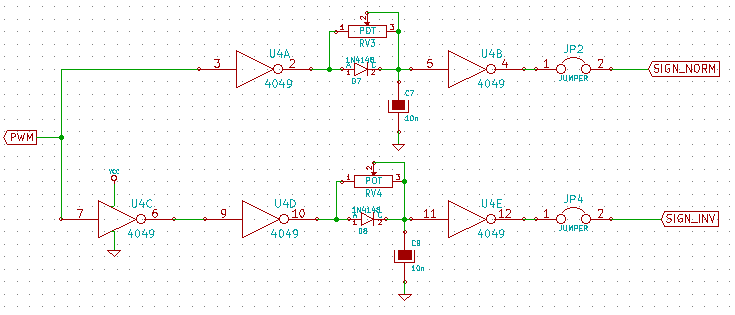
\includegraphics[width=13cm]{Imagenes/circ_retardo.png}
	\caption{Circuito de Retardo}
	\label{fig:circ_retardo}
\end{figure} 


\subsection{Protección}\label{sec:proteccion}

Para proteger el circuito de sobre corrientes, incluimos el bloque de protección detallado en la Figura \ref{fig:circ_protecc}.

A la salida del puente H, en serie con el motor, colocamos una resistencia sensora con el objetivo de medir la corriente que circula por el motor. Esta tensión medida, equivalente a la corriente, es comparada con una referencia fijada por un potenciómetro. A la salida del comparador, la señal resultante activa el pin de Shutdown \textit{sh\_dw} de los drivers.

Cuando la tensión en la resistencia sensora supera la tensión de referencia, la salida de comparador entrega una tensión equivalente a un 1 lógico que dispara el SCR poniendo en conducción el transistor BC558 que activa el pin de apagado de los IR2110, derivando en una inmediata interrupción de la alimentación de los motores. Gracias al circuito de enclavamiento generado por el SCR, es necesario interrumpir la excitación del transistor mediante el pulsador $SW1$ para que el SCR se apague y el motor vuelva a funcionar.

Para calibrar la protección se coloca el motor a girar a las revoluciones deseadas y se calibra para que, al aplicar fuerza extra sobre el eje, la protección se active. Esto garantiza un margen de corriente en el que el funcionamiento sea normal y que al aumentar la corriente, por un esfuerzo extra, la protección se active.


\begin{figure}[h]
	\centering
	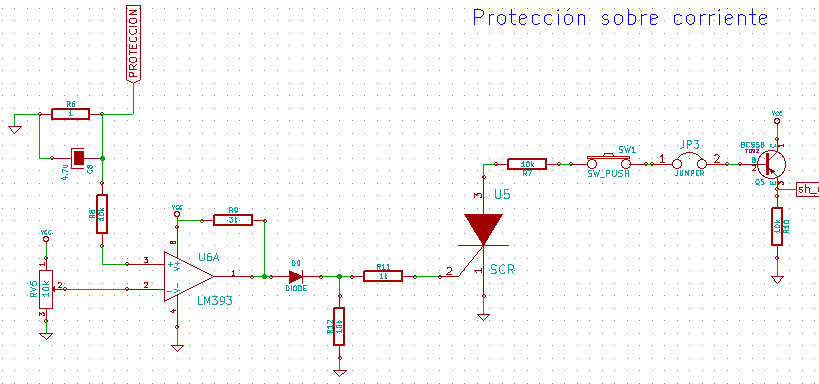
\includegraphics[width=13cm]{Imagenes/circ_prot.png}
	\caption{Circuito de Protección}
	\label{fig:circ_protecc}
\end{figure} 

\section{Mediciones}

En la Figura \ref{fig:osc_max} se observa el PWM obtenido para la condición de máxima velocidad del motor. En ella se puede apreciar los tiempos muertos entre ambas señales y el concepto del toque constante. 

Por otro lado, en la Figura \ref{fig:osc_min} ambas señales poseen un dutty cycle del 50\%, lo que provoca que el motor se detenga pero mantenga el torque.

\begin{figure}[h]
	\centering
	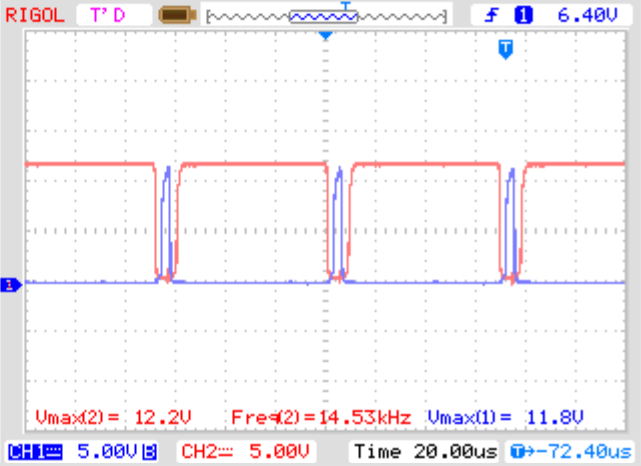
\includegraphics[width=9.5cm]{Imagenes/osc_max.png}
	\caption{PWM para motor a máxima velocidad}
	\label{fig:osc_max}
\end{figure} 



\begin{figure}[h]
	\centering
	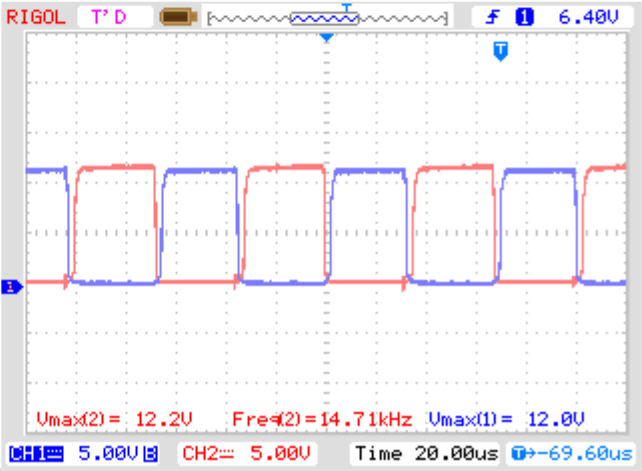
\includegraphics[width=9.5cm]{Imagenes/osc_min.png}
	\caption{PWM para detención del motor}
	\label{fig:osc_min}
\end{figure} 

\subsection{Volts vs RPM}
Mediante la utilización de un sensor infrarrojo y un marcador en el eje del motor procedimos a medir la relación entre la tensión de entrada al generador de PWM y las revoluciones por minuto obtenidas en el motor.

Para la relevación de las mediciones, barrimos manualmente el rango de funcionamiento de generador de señal y midiendo la frecuencia de los pulsos a la salida del sensor. Cada pulso negativo corresponde al momento en el que el sensor se veía obstruido por el marcador, por lo que la frecuencia en hertz obtenida es el equivalente a las RPS. Para obtener las RPM se multiplicó la medición por 60 segundos.

Los valores obtenidos fueron los siguientes:

%\begin{table}[]
%	\centering
%	\caption{Tensión vs RPM}
%	\label{my-label}
%	\begin{tabular}{l|l|l}
%
%
%Vref & Frec & RPM\\
%3,5	& 59,52	& 3571,2\\%
%3,4	& 53,19	& 3191,4\\
%3,3	& 48,1	& 2886\\
%3,2	& 42,37	& 2542,2\\
%3,1	& 37,8	& 2268\\
%3	& 31,65	& 1899\\
%2,9 & 25,51	& 1530,6\\
%2,8	& 19,69	& 1181,4\\
%2,7	& 14,53	& 871,8\\
%2,6	& 8,9	& 534\\
%2,5	& 2,8	& 168\\
%2,4	& 0	& 0\\
%1,9	& 0	& 0\\
%1,8	& 4,2	& 252\\
%1,7	& 6,3	& 378\\
%%1,6	& 11,63	& 697,8\\
%1,5	& 17,86	& 1071,6\\
%1,4	& 23,58	& 1414,8\\
%1,3	& 30,49	& 1829,4\\
%1,2	& 40,32	& 2419,2\\
%1,1	& 50	& 3000\\
%1	& 59,52	& 3571,2\\
%0,9	& 63,29	& 3797,4 \\
%	\end{tabular}
% \end{table}

\begin{figure}[h]
	\centering
	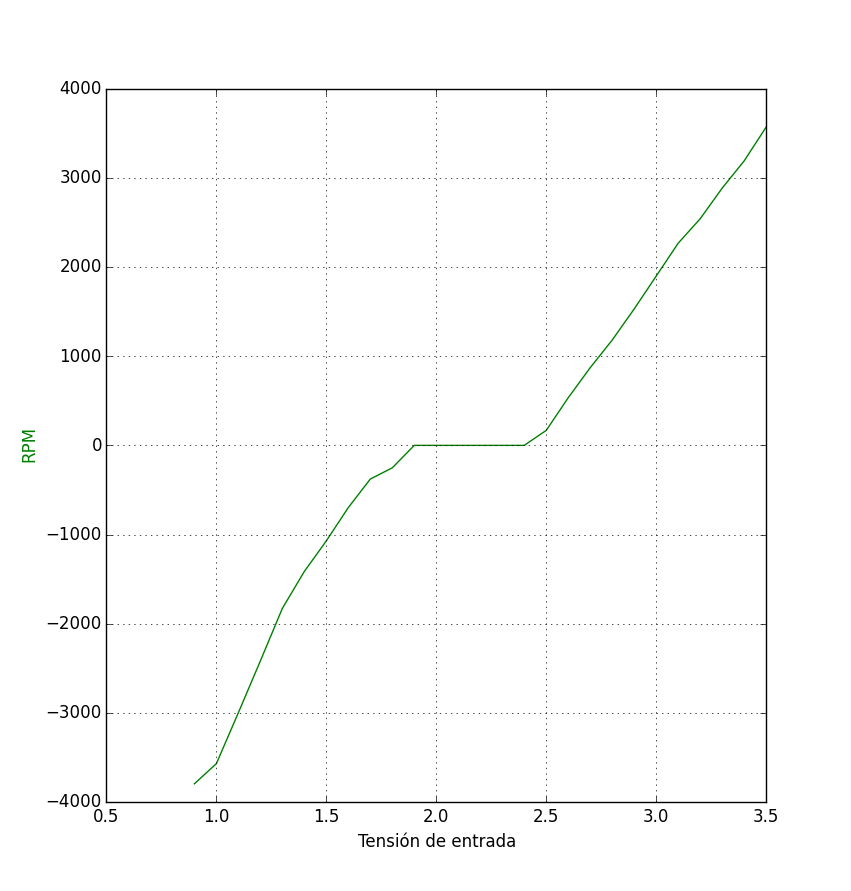
\includegraphics[width=15cm]{Imagenes/rpm.png}
	\caption{Curva de Tensión vs RPM}
	\label{fig:rpm}
\end{figure} 


\subsection{Protección}
Se ajustó la tensión de referencia en un valor tal que al forzar el motor, el circuito actuara y lo detuviera. La protección funcionó tal y como se esperaba, deteniendo la marcha hasta el momento en el que se presionó el pulsador de liberación.


\section{Conclusiones}
La implementación del circuito conllevó una dificultad mínima, logrando muy buenos resultados. El puente H resulta muy útil para controlar no solo la velocidad de giro, si no también el sentido de giro y lograr una frenada instantánea.

En este práctico, la señal de PWM la obtuvimos de un circuito integrado, controlando la velocidad mediante una señal de referencia, pero este circuito podría ser reemplazado por un microcontrolador y controlar la velocidad del motor digitalmente.

La separación del circuito en módulos permite la fabricación y prueba de los sub circuitos por separado. En nuestro caso utilizamos la protección por sobre corriente actuando sobre la pata de shutdown del driver, pero podríamos haber utilizado una implementación equivalente sobre la alimentación del circuito. Una variación al circuito de protección fue el agregado del SCR, que permite una mayor seguridad no volviendo a encender el motor hasta la intervención de un operario.

El potenciómetro nos permite ajustar el nivel de referencia para poder cambiar el nivel de protección, siendo capaces de ajustarlo al tipo de motor y a las necesidades de la aplicación

Al observar la curva de la relación Tensión - RPM, vemos un valle al cruzar por 0. Esto lo relacionamos al tamaño del motor, ya que un motor de tales dimensiones posee un umbral de tensión elevado para comenzar a moverse.


\end{document}
>>>>>>> 9d12e934d1c1893bb0400a79f64badcfbee4410f
